\section{The benchmark}
\label{sec:benchmark}

The benchmark serves a learner a stream of ARC task instances and charges it for the feedback it uses. We define streams for ARC-AGI-1, ARC-AGI-2 and ARC-AGI-3. We focus here on ARC-AGI-1, with preliminary results for the other two editions in Appendix~\ref{app:tracks}.

\Needspace{16\baselineskip}  %
\subsection{One instance}
\label{sec:interface}

\begin{wrapfigure}[14]{r}{0.46\linewidth}
\vspace{-11pt}  %
\centering
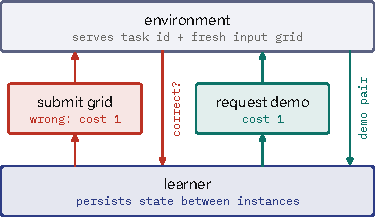
\includegraphics[width=\linewidth]{figures/protocol.pdf}
\caption{Each incorrect attempt or demonstration costs one. Unsolved instances cost the full budget of sixteen.}
\label{fig:protocol}
\vspace{\dimexpr\baselineskip-8pt\relax}  %
\end{wrapfigure}
An ARC task is a rule that turns an input grid into an output grid, and an instance of it is one input whose output the learner must produce. For each instance, the learner observes the task id, the input grid, and how many attempts and demonstration requests it has used on the instance thus far, but it is told nothing about its position in the stream. It may submit a grid, and the environment answers only correct or incorrect. A correct submission ends the instance, and an incorrect one costs $c_w = 1$. It may instead request a demonstration, at a cost of $c_d = 1$, which returns one more input-output pair of the task, up to eight per instance (Figure~\ref{fig:protocol}). A ninth demonstration request in the same instance is refused and costs nothing. An instance ends on a correct submission or on the eighth wrong attempt, and the learner cannot abandon it. Failing to get the correct answer costs 16, even if there were demonstration requests to spare. We deliver the verdict on the final submission before any storage step, such that storage decisions can reflect the outcome.

Let $w_{\max} = 8$ be the attempt cap and $d_{\max} = 8$ the demonstration cap, and on instance $i$ let $s_i \in \{0, 1\}$ say whether it was solved, $w_i$ be the wrong submissions and $d_i$ the demonstration requests. We express each instance's charge $c_i$ as a percentage $u_i$ of the budget cap $C_{\max}$. For a set of instances $\mathcal{I}$, the mean budget used $U(\mathcal{I})$ averages these percentages, and the solve rate $P(\mathcal{I})$ is the percentage of instances solved:
\begin{equation}
\begin{gathered}
c_i = \begin{cases} c_w w_i + c_d d_i & s_i = 1 \\ C_{\max} & s_i = 0 \end{cases}, \qquad C_{\max} = c_w w_{\max} + c_d d_{\max} = 16, \qquad u_i = 100\, \frac{c_i}{C_{\max}}, \\
U(\mathcal{I}) = \frac{1}{|\mathcal{I}|} \sum_{i \in \mathcal{I}} u_i, \qquad P(\mathcal{I}) = \frac{100}{|\mathcal{I}|} \sum_{i \in \mathcal{I}} s_i.
\end{gathered}
\label{eq:score}
\end{equation}
For example, a solved instance with charge $c_i=4$ uses $u_i=25$\% of its budget, and an unsolved instance has $c_i=16$ and $u_i=100$\%. A set containing only those two instances has $U=62.5$\% and $P=50$\%. For a single instance, $U(\{i\})=u_i$. Because a failure costs the whole budget however it came about, failing is never cheaper than asking, and a demonstration is paid for only by an instance it helped to solve. We take $U$ as the raw measure (lower is better), and quote $P$ beside it, given that neither number determines the other, and the two are complementary.

We keep the feedback binary, as ARC Prize does and as a deployed system experiences it, since returning the correct grid on failure would turn the stream into supervised learning. We also expose the task id on every instance, under an alias drawn for each run, to enable the system to properly disambiguate between tasks, as the input grid is not a unique identifier for the task. See Appendix~\ref{app:bench}.

\subsection{A stream of instances}
\label{sec:stream}

\begin{figure}[t]
\centering
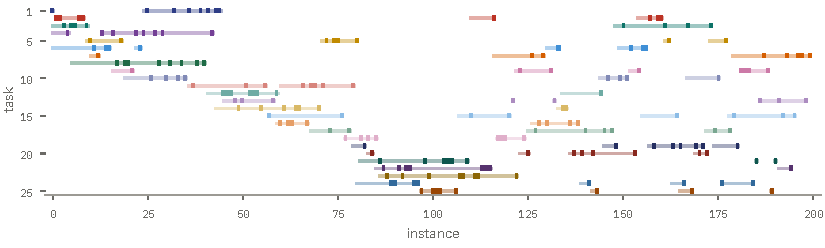
\includegraphics[width=\linewidth]{figures/modes.pdf}
\caption{The ARC-AGI-1 stream: its 25 tasks, one row each in the order they first appear, and each instance a mark. A thin line in the task's color marks a spell in which the task is active.}
\label{fig:modes}
\end{figure}

A learner meets instances as a stream of consecutive rounds, each naming a task and an instance seed (one per user, Section~\ref{sec:regimes}). At round $t$, an active set $\mathcal{A}_t$ holds at most $n_c$ tasks, from which the round's task $\tau_t$ is drawn uniformly. A task that enters the active set stays for a spell of $\beta$ instances, after which it rests for $\rho$ instances before it may return. Never-seen tasks arrive every $\alpha$ instances and take the next free place:
\begin{equation}
\tau_t \sim \mathrm{Unif}(\mathcal{A}_t), \qquad \beta \sim \mathrm{Exp}(b), \qquad \rho \sim \mathrm{LogNormal}(\ln m, \sigma), \qquad \alpha \sim \mathrm{Exp}(a).
\label{eq:stream}
\end{equation}
We round spells and rests to whole instances, and each is at least one, see Algorithm~\ref{alg:stream} in Appendix~\ref{app:schedules}. The stream keeps a few tasks active at once, each worked in bursts with dormant gaps between them, see Figure~\ref{fig:modes}. A task can stay dormant for long enough to be forgotten, and since every instance is a fresh draw from the task's generator, no answer can be cached.

On ARC-AGI-1, the stream draws 25 of the 400 training tasks and serves 200 fresh, verified instances of them from the Re-ARC generators \citep{hodel2024rearc}, and a held-out test after the stream draws on the 400 evaluation tasks. Four tasks are active at once, spells last about three instances and rests about thirty, and a new task arrives about every four instances, the last in round 97 (Table~\ref{tab:configs} in Appendix~\ref{app:bench}). Every task serves eight instances, after which it is finished. Each ARC-AGI edition has one fixed stream and fixed tests; other seeds draw other streams from the same process (Appendix~\ref{app:schedules}), and all results quoted use a seed of 0. Every system therefore meets the same tasks in the same order, with the same instances. The streams on ARC-AGI-2 and ARC-AGI-3 \citep{chollet2025arcagi2,arcprize2026arcagi3} serve fresh instances from generators of their own. Figures~\ref{fig:plane-arc2} and~\ref{fig:plane-arc3} in Appendix~\ref{app:tracks} are deliberately sparse, leaving these harder tracks open for the community's new methods and submissions, with the directions we find most promising presented in Section~\ref{sec:discussion}.

\subsection{Two tests after the stream}
\label{sec:tests}

The stream measures what a learner keeps while it learns. To measure what it has at the end, we freeze the learner and serve it two tests, each a single round of 100 instances. The learner is not told that a test has begun. We start every test instance from the learner's state at the end of the stream, and nothing learned on one test instance reaches another. The seen test consists of four fresh instances of each of the stream's 25 tasks, at instance seeds the stream did not use, and measures memorization. In the held-out test, which measures generalization, 100 evaluation tasks never seen on the stream are served once each. A learner that keeps one program per task gets cheaper on the seen test but no cheaper on the held-out test, whereas a learner that has become a better solver of new tasks gets cheaper on both. Plotting the two tests against each other (Figure~\ref{fig:plane}) is the continual counterpart of plotting in-distribution against out-of-distribution accuracy \citep{miller2021accuracy}.

\subsection{Measuring learning}
\label{sec:metrics}

$U$ over the stream mixes what a learner could already do before the stream with what it learns along the way. To measure the learning alone, we need one more run, the \emph{reset}: the same learner on the same stream and the same tests, with its state wiped before each instance. Let $U_{0}(\mathcal{I})$ be the reset's budget used over the stream's instances $\mathcal{I}$, and $U^{*}(\mathcal{I})$ that of perfect memory on the same system, which pays the reset's own charge on each task's first exposure and nothing on any return. The learnable budget $\Lambda = U_{0}(\mathcal{I}) - U^{*}(\mathcal{I})$ is the most any memory can save, giving the share learned:
\begin{equation}
L = \frac{U_{0}(\mathcal{I}) - U(\mathcal{I})}{\Lambda}.
\label{eq:learned}
\end{equation}
It is 0 for a learner that keeps nothing, 1 for one that answers every returning task at no cost, and negative for one that does worse than the reset. $L$ therefore measures learning alone, with base capability normalized out. On each of the two tests after the stream, the best a learner can spend is nothing, so we read the same saving as a share of the reset's whole spend on the test's instances $\mathcal{E}$:
\begin{equation}
S = \frac{U_{0}(\mathcal{E}) - U(\mathcal{E})}{U_{0}(\mathcal{E})}.
\label{eq:transfer}
\end{equation}
We write the share saved on the seen test as $S_{\mathrm{seen}}$ and on the held-out test as $S_{\mathrm{held}}$. Taking it as a share of the reset's spend means that a learner whose reset already spends little is not marked down for having less to save. On the seen test, whose tasks the stream has met, $S_{\mathrm{seen}}$ measures memorization. On the held-out test there is nothing to remember, so $S_{\mathrm{held}}$ measures generalization, how much better a learner has become at tasks it never met. The learner plays each whole test \testPlays{} times from where the stream left it, and the reset \testPlays{} times from nothing, on the same instances. Averaging each instance's \testPlays{} plays smooths out the model's random sampling, and $S$ is computed from these averages. We give $L$, $S_{\mathrm{seen}}$ and $S_{\mathrm{held}}$ with 95\% intervals over tasks (Appendix~\ref{app:bench}).

\subsection{Two regimes: the individual and the collective}
\label{sec:regimes}

So far, on the stream, a single system meets one instance at a time, and whatever it carries may change between any two instances. A deployed system may instead serve many people at once, learning from \emph{all} of them, and the collective regime tests such a system. A run has $n_u \in \{1, 2, 4\}$ users, each following a separate stream over 25 non-overlapping tasks, so that two users bring 50 unique tasks and four bring 100. A round serves one instance per user, concurrently, and the system may change its state only between rounds. Any learner can run in either regime, whether it keeps notes or updates its weights. Each user's tasks still arrive and go dormant, and every round is charged (Appendix~\ref{app:schedules}, and Table~\ref{tab:configs} in Appendix~\ref{app:bench}). All users share one state, both the harness's notes and the trained model's weights, so that whatever a learner keeps, it learns from every user's games. With more than one user, the seen test spreads its 100 instances over every user's tasks (Appendix~\ref{app:schedules}).

\subsection{Verifying a result}
\label{sec:tracks}

Every task of the benchmark and every task's solver presented so far is public. External submissions are therefore verified by running the learner's code on a private set of 50 new rules that only we have seen (Appendix~\ref{app:heldout}): 25 for the stream and the seen test, and 25 for the held-out test. For now this verifies a learner at one user, and we will soon add rules for the collective regimes. A learner is verified automatically from an issue on the benchmark's repository. Continual-ARC is designed to explain how a learner learns rather than to purely rank learners, so we give no single score per se. For illustration, reducing budget use from 2\% for the reset to 1\% for the learner saves half the reset's spend, but only one percentage point of the full budget. Reducing it from 100\% to 90\% saves 10\% of the reset's spend, yet still consumes 90\% of the full budget. We therefore present all verified submissions of genuine learning algorithms on the benchmark, with Figure~\ref{fig:plane} showing the canonical representation.
